\chapter{Решение на основе \texttt{Moflow gentrace}}

\section{Устройство оригинального инструмента}

Прежде всего, следует подробнее разобраться как устроен и работает \texttt{gentrace}. Для начала, на примере где все работает корректно.

Пусть некоторый файл был отмечен как источник помеченных данных, тогда при первом чтении этого файла при помощи системного вызова \texttt{read(fd, buf, 10)} будут созданы метки с номерами от $1$ до $10$ и поставлены в соответствие ячейкам памяти $\texttt{buf[0]}\ldots \texttt{buf[10]}$ соответственно. Пусть затем была выполнена инструкция \texttt{cmp rax, buf+0x9}, регистр \texttt{RFLAGS} становится помеченным меткой $10$, соответсвенно послудеющий условный переход зависит от $10$ байта.


\begin{figure}[H]
    \center{
        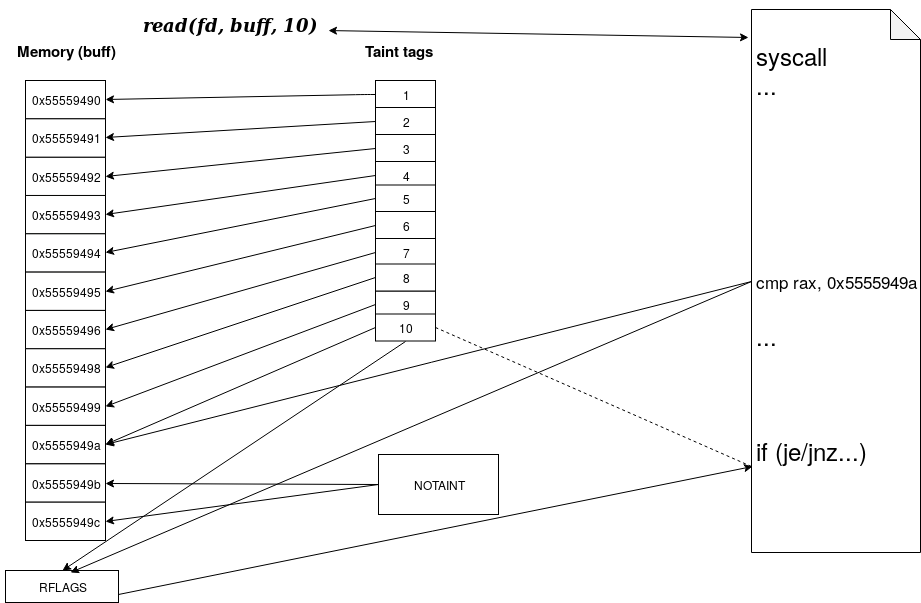
\includegraphics[scale=0.5]{img/source_tainting.png}
    }
    \caption{Создание пометок в \texttt{moflow gentrace}}
    \label{fig:moflow1}
\end{figure}

Теперь рассмотрим другой случай. Пусть после вызова \texttt{read(fd, buf, 10)} последует инструкция \texttt{mov rcx, qword ptr [rsi]}, где \texttt{rsi} хранит адрес \texttt{buf}. В то время как в действительности произошло побайтовое копирование, \texttt{moflow} видит это иначе.

\begin{itemize}
    \item Для каждого адреса или регистра, который читается в рамках инструкции берется соответсвуюшая ему метка. Все полученные метки объединяются при помоши функции \texttt{combineTaint}.
    \item В каждый адрес или регистр, в которых во время инструкции происходит запись пишется метка, полученная в предыдущем пункте.
\end{itemize}

\begin{lstlisting}[environoment=cpp_code,captionpos=b]
uint32_t TaintTracker::combineTaint(uint32_t oldtag, uint32_t newtag)
{
  if (newtag) {// its tainted
    if (oldtag == NOTAINT)
      return newtag; // FIXME
    else 
      return MIXED_TAINT;
  }
  return oldtag;
}
\end{lstlisting}

Гдe \texttt{NOTAINT} это $0$ -- значение обозначающее, что метка отсутствует, а \texttt{MIXED\_TAINT} это $2^{32}-1$, обозначающее наличие более чем одной пометки.

\begin{figure}[H]
    \center{
        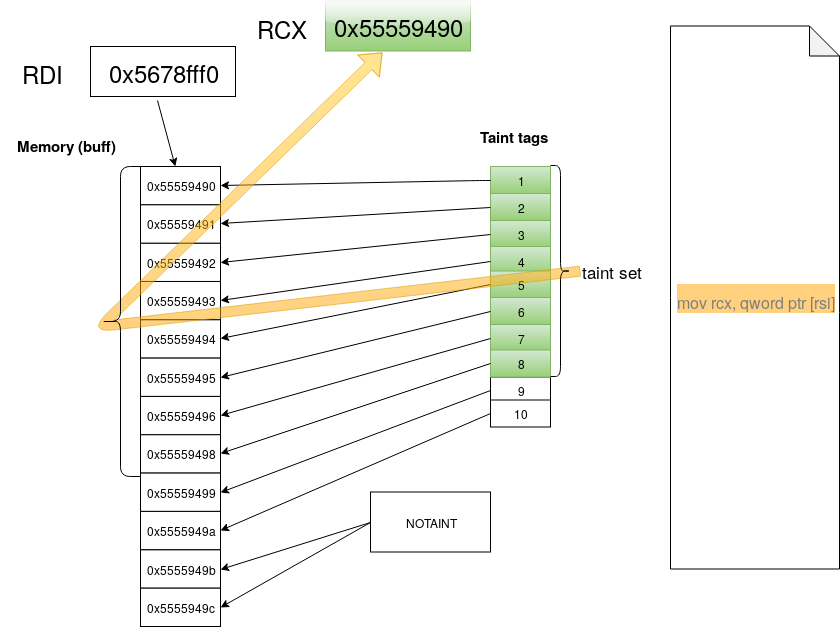
\includegraphics[scale=0.5]{img/propagation1.png}
    }
    \caption{Распространение пометок в \texttt{moflow gentrace}}
    \label{fig:moflow2}
\end{figure}

Таким образом, первое что необходимо реализовать это структуру \texttt{Множество меток}, которая должна поддерживать $3$ операции.

\begin{itemize}
    \item Добавление метки в \texttt{множество меток}.
    \item Объединение с другим \texttt{множество меток}
    \item Вывод содержимого Множества \texttt{множества меток}
\end{itemize}

Предположим теперь, что эта структура уже есть (далее будут описана её реализация). Допустим, встретилась еще одна инструкция копирования \texttt{mov word ptr [rdi], rcx}. \textbf{0x5678fff0} и \textbf{0x5678fff1}помечаются $8$ тэгами. Правильно было бы представить \textbf{RCX} как 8 отдельных байт, которые могут быть помечены независимо, тогда \textbf{0x5678fff0} и \textbf{0x5678fff1} будут помечены $2$ различными тегами.

\begin{figure}[H]
    \center{
        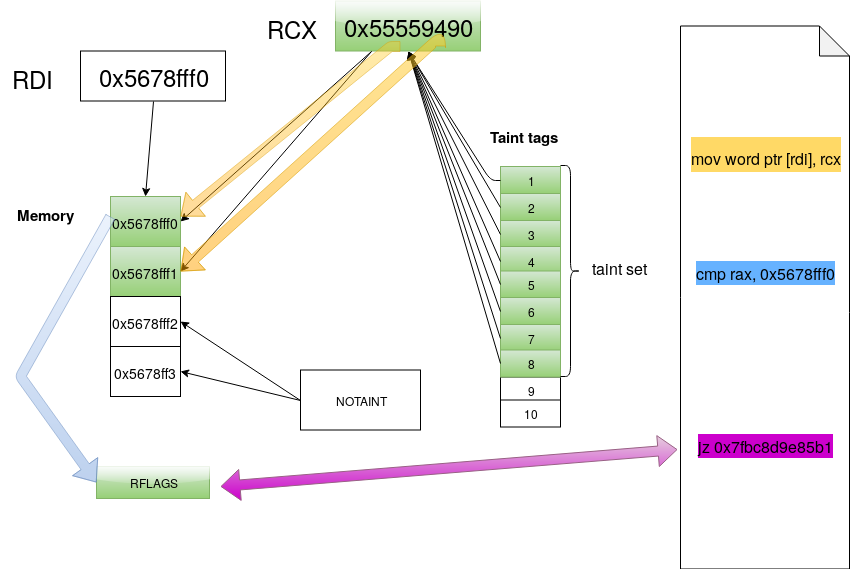
\includegraphics[scale=0.5]{img/propagation2.png}
    }
    \caption{Перепомечивание в \texttt{moflow gentrace}}
    \label{fig:moflow3}
\end{figure}

\section{Реализация \textt{Множества Пометок}}

Наиболее простым и естественным решением, было бы использовать структуру данных реализующую интерфейс обычного множества в математическом смысле, в случае \texttt{C++} такой структурой данных является \texttt{std::set}. Тем не менее, непосредственные попытки использования вызвали ощутимые проблемы в производительности. Профилирование показало, что проблема в многочисленных аллокациях памяти, связанных c

\begin{itemize}
    \text Операцией объединения множеств
    \text Многочисленными аллокациями, вызванными необходимостью создавать временные множества пометок на каждую операцию распространения пометок
\end{itemize}

Дальнейший анализ показал, что на всех изученных примерах более чем в 70\% случаев соответствуюшие адресам и регистрам \texttt{множества пометок} оказываются пустыми или состоящими из одного элемента. Отсюда вытекает очевидная оптимизация. Будем представлять множество пометок в виде типа-суммы из двух элементов: \texttt{uint32\_t} и \texttt{tag\_set*}, где первый элемент используется как в оригинальном \texttt{gentrace}, то есть говорит об отсутствии метки, наличии единственной метки (в этом случае содержит её значение) или показывает, что меток более чем одна. В последнем случае используется непосредственно \texttt{tag\_set*}, в иных случаях значением второго элемента является нулевой указатель.

Не смотря на приведенную выше оптимизацию, остатеся необходимость реализовать структуру реализующую само множество. Были рассмотренны следующие варианты.

\bigskip

Использование обычного \texttt{std::vector}. При этом 
\begin{itemize}
    \item Добавлению соответствует операция добавления элемента в конец вектора.
    \item Обьединению запись второго вектора в конец первого, с последующим удалением дублирующих элементов\footnote{Были проведены эксперименты, для определения границы при превышение которой стоит начать удаление дублей. Результаты показали, что разница между порог в 20 элементов и меньшими статистически не различима, в то время как большие значение показывают худший результат}
    \item Вывод значений производится итерацией по элементам вектора.
\end{itemize}

\bigskip

Использование битового множества фиксированного размера \texttt{std::bitset}. Поскольку количество элементов должно быть известно на этапе компиляции, этот подход в чистом виде не применим. Тем не менее он представляет интерес как некоторые ориентир, в тестах было использовано значение в $6000$, как наименьшее круглое значение которого достаточно для тестовых примеров.
При данном подходе для всех операций использовался естественный интерфейс битового множества.

\bigskip

CRoaring -- реализация протокола сжатых битовых векторов \texttt{Roaring} \cite{Roaring}. Данная библиотека в целом аналогична обычному битовому множеству с точки зрения интерфейса, однако поддерживает операции над множествами разного размера. Реализация также использовала естественный интерфейс множества, предлагаемый библиотекой.

\bigskip
Использование множества битовых векторов фиксированного размера.

\bigsckip
Использование библиотеки множеств интервалов (\texttt{boost::icl::interval\_set}).

\textbf{Время работы в секундах для различных реализаций}\\
    \scalebox{0.75}{
    \begin{tabular}[]{@{}llllllll@{}}
    \toprule
    & vanilla & vector & bitset6000 & roaring & bitset64 tree & bitset256
    tree & bitset512 tree\tabularnewline
    \midrule
    % \endhead
    cmark & 3.5s & 4.6s & 3.7s & 4.2s & 3.8s & 3.7s & 3.7s\tabularnewline
    file & 20.8s & 47s & 60s & 70s & 45.5s & 46.3s & 47.5s\tabularnewline
    libjpeg & 14.5s & 1762s & 49s & 378s & 307s & 108s & 80s\tabularnewline
    libyaml & 16.5s & 22.5s & 25s & 26s & 23.5s & 23.5s & 23.5s\tabularnewline
    \bottomrule
\end{tabular}}

\section{Другие доработки}
